\documentclass[a4paper,11pt,titlepage]{article}

\usepackage{latexsym}
\usepackage{graphicx}
\usepackage{float}
\usepackage{url}
\usepackage{unicode}
\usepackage[polish]{babel}
\usepackage{titlesec}

\newcommand{\sectionbreak}{\clearpage}
\author{Adam Talarczyk}
\title{Projektowanie aplikacji mobilnych}
\frenchspacing
\begin{document}
\begin{titlepage}
    \begin{center}
        \vspace*{1cm}
 
        \Huge
        \textbf{Projektowanie aplikacji mobilnych}
 
        \vspace{0.5cm}
        \LARGE
        ``AirQuality''


 Odczyt jakości powietrza ze stacji pomiarowych
 
        \vspace{1.5cm}
 
        \textbf{Adam Talarczyk}
 
        \vfill
 
        \vspace{0.8cm}
 
        \Large
        Wydział Nauk Ścisłych i Technicznych

        Uniwersytet Śląski

	Semestr letni 2020/2020
 
    \end{center}
\end{titlepage}
\newpage
\tableofcontents
\newpage

\section{Wstęp}
\subsection{Założenia projektowe}
Głównym zalożeniem aplikacji jest pobieranie danych ze stacji pomiarowych oraz wyświetlanie ich w czytelny dla użytkownika sposób. Aplikacja przewiduje wyszukiwanie stacji na mapie, dodawanie lub usuwanie ich z zakładek, oraz prezentacja wybranych stacji na stronie głównej. Dane dostarczane przez aplikację pochodzą z publicznego interfejsu programistycznego aplikacji (https://powietrze.gios.gov.pl/php/content/api), który udostępnia wyniki automatycznych pomiarów dwutlenku siarki (SO2), dwutlenku azotu (NO2), pyłu PM10, pyłu PM2,5, tlenku węgla (CO), benzenu (C6H6), ozonu (O3). Dodatkowo, gdy poziom zanieczyszczenia powietrza dla najbliższej stacji pomiarowej przekroczy normę, aplikacja poinformuje o tym użytkownika przy pomocy powiadomienia.

Aplikacja przeznaczona jest wyłącznie na smartfony firmy Apple. Napisana została w języku Swift przy użyciu narzędzia Xcode.
\subsection{Wymagania funkcjonalne}
\begin{itemize}
 	\item Wyświetlanie na mapie wszystkich stacji pomiarowych na terytorium polski
  	\item Dodanie stacji pomiarowej do zakładek
  	\item Usuniecie stacji pomiarowej z zakładek
	\item Wyświetlenie szczegółowych pomiarów wybranej stacji
	\item Wyświetlanie najbliższej stacji pomiarowej w lokalizacji użytkownika
	\item Obsługa trybu nocnego
\end{itemize}
\subsection{Wymagania niefunkcjonalne}
\begin{itemize}
 	\item Aplikacja automatycznie odświeża dane o pełnej godzinie (wynika to ze sposobu działania API)
	\item Działanie aplikacji oraz czas pobierania danych ograniczone są do przepustowości interfejsu programistycznego
	\item Komunikacja z serwerem API odbywa się poprzez protokół HTTP
	\item Interfejs użytkownika zaprojektowany jest zgodnie z wytycznymi Apple przy pomocy frameworku UIKit
	\item Pobieranie oraz aktualizacja lokalizacji użytkownika
\end{itemize}

\section{Specyfikacja zewnętrzna}
\subsection{Instrukcja obsługi}
Użytkownik po uruchomieniu aplikacji i zaakceptowaniu komunikatu o usłuchach lokalizacji znajduje się na stronie głównej, na której na samym początku widzi tylko najbliższą w okolicy stację pomiarową (zakładka z niebieskim tłem wyszczególniona na ryskunku nr. 1). Na dolnym pasku nawigacji ma on do dyspozycji:
\begin{itemize}
 	\item Stronę główną (na której się znajduje)
	\item Mapę
	\item Ustawienia
\end{itemize}


\begin{figure}[H]
\centering
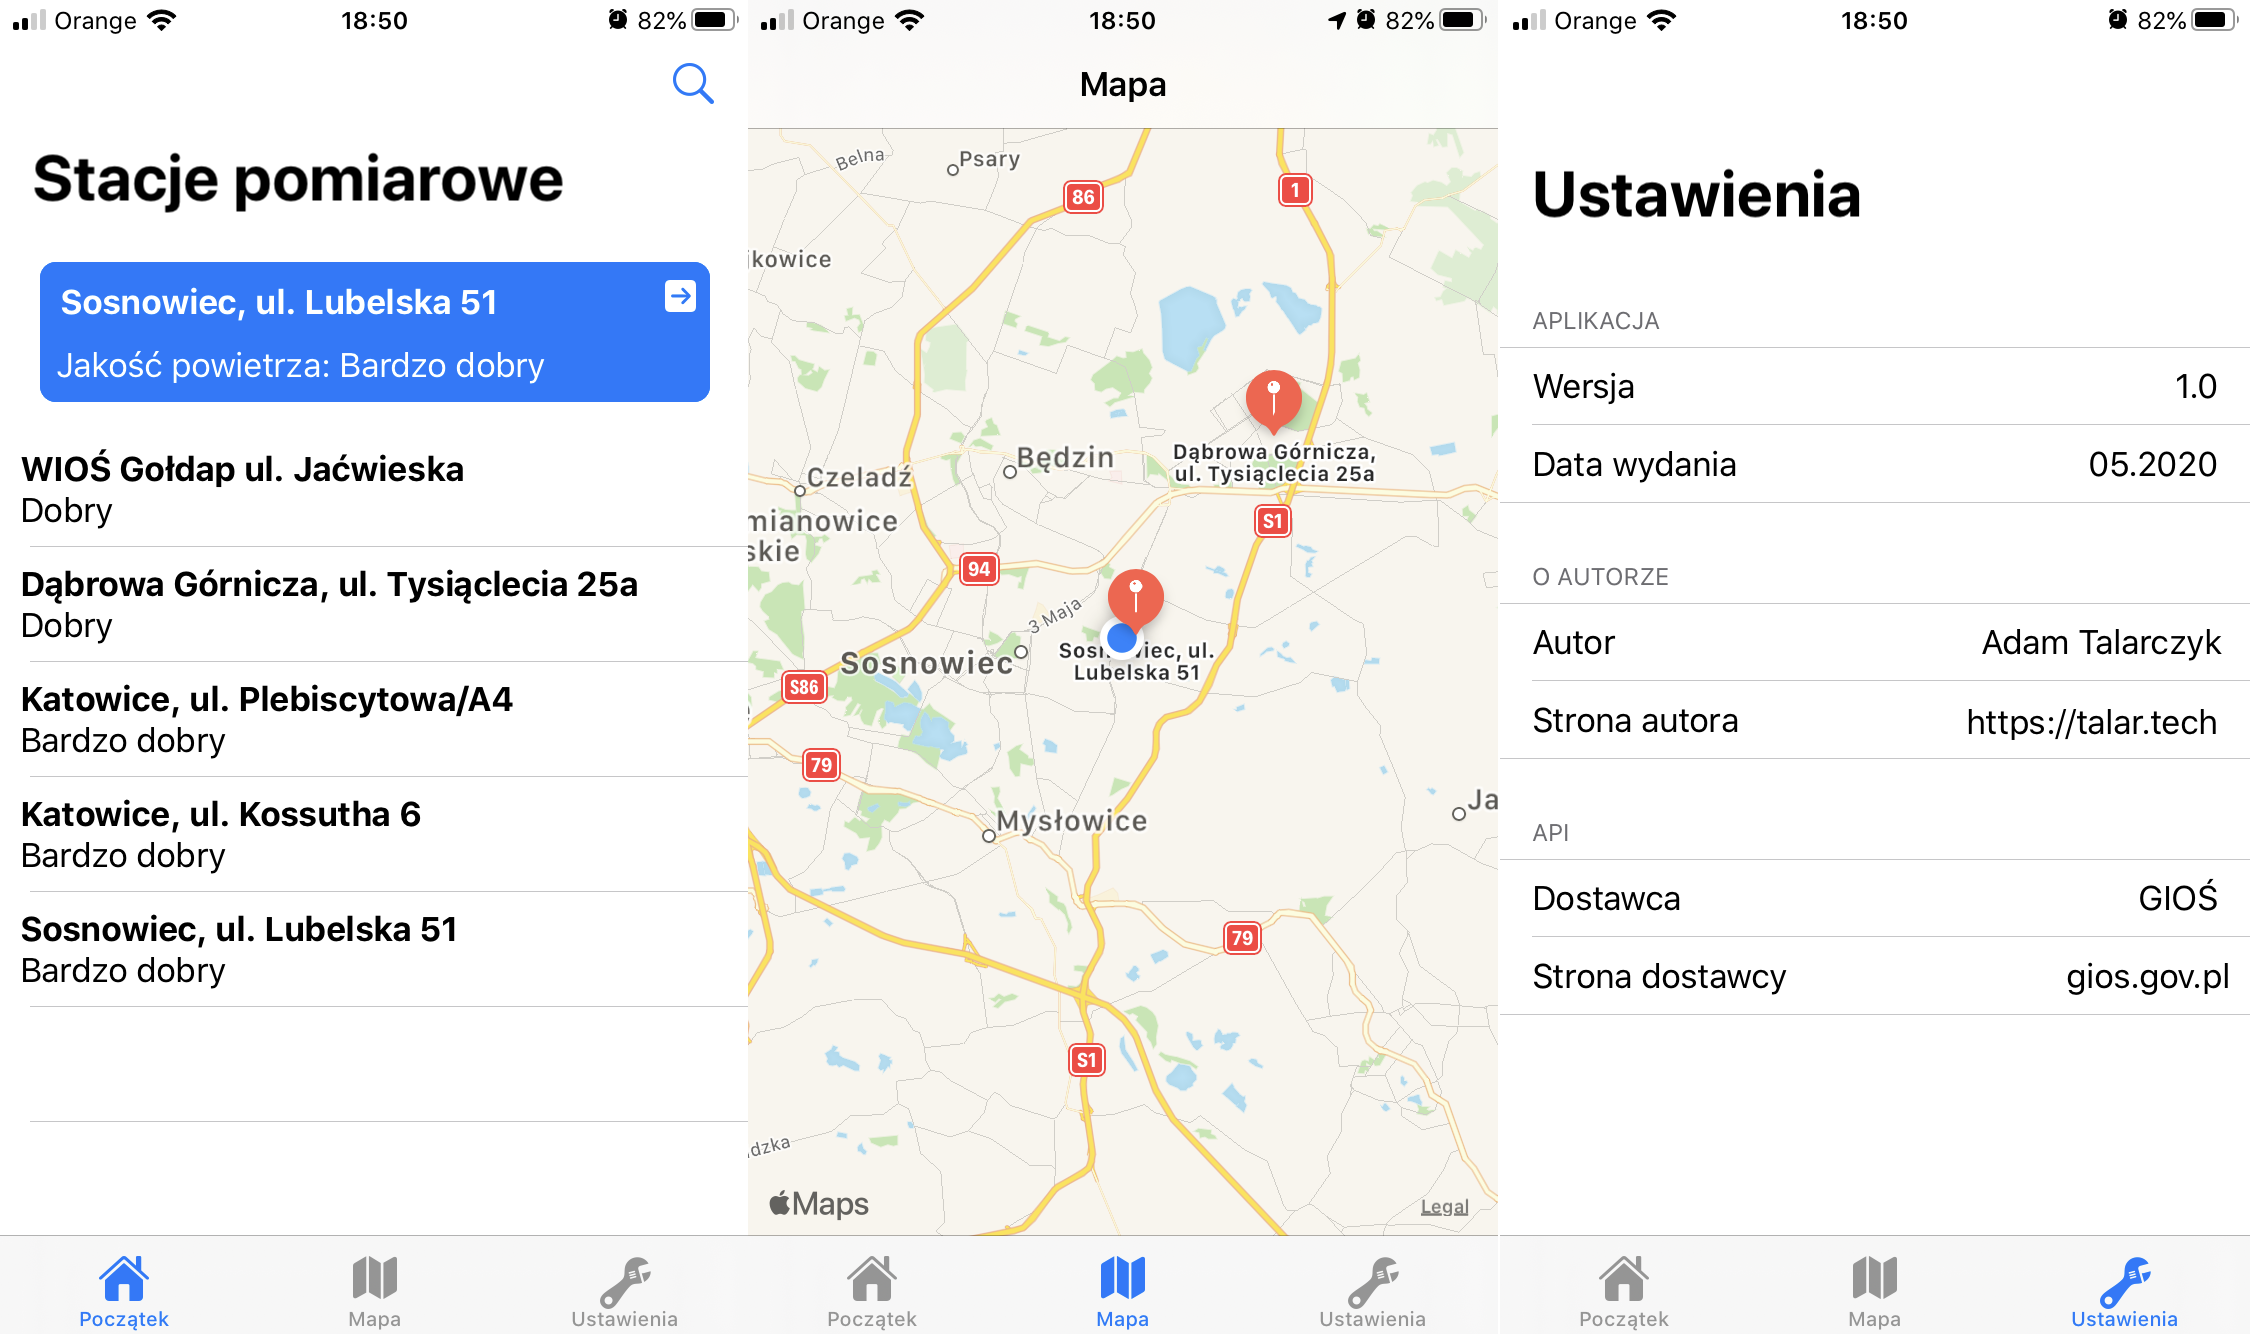
\includegraphics[width=1\columnwidth]{img/img1.PNG}
\caption{Wygląd zakładek: strony głównej, mapy oraz ustawień} 
\end{figure}

Po kliknięciu w zakładkę mapy zostanie przeniesiony do widoku, gdzie na mapie zaznaczone punktami są wszystkie dostępne stacje pomiarowe wraz z ich nazwą. Użytkownik może oddalać, przybliżać oraz przesuwać się po mapie. Jego lokalizacja również jest uwzględniona (z dokładnością do 1 kilometra w celu zminimalizowania użycia energii). Po kliknięciu w punkt ze stacją otwarte zostają szczegóły stacji pomiarowej, gdzie znajdują się wszystkie informacje o sensorach oraz pomiarach. Użytkownik może dodać stację pomiarową do zakładek, wówczas na stronie głównej zaraz pod najbliższą w okolicy stacją zostają wyświetlone wszystkie stacje z zakładek.

Użytkownik może również wyszukać stację po jej nazwie (która zazwyczaj zawiera nazwę miasta). W tym celu trzeba wejść na stronę główną i w prawym górnym rogu kliknąć przycisk lupy. Otworzy się wówczas widok z listą wszystkich stacji pomiarowych (około 190). By zainicjować wyszukiwanie trzeba przejechać palcem od góry do dołu, wtedy wyświetli się pasek wyszukiwania, w którym wpisać można odpowiednią frazę. Wybór stacji, tak jak w przypadku zakładki mapy otworzy nam widok ze szczegółami. Możemy zaobserwować to na rysunku nr. 2.

\begin{figure}[H]
\centering
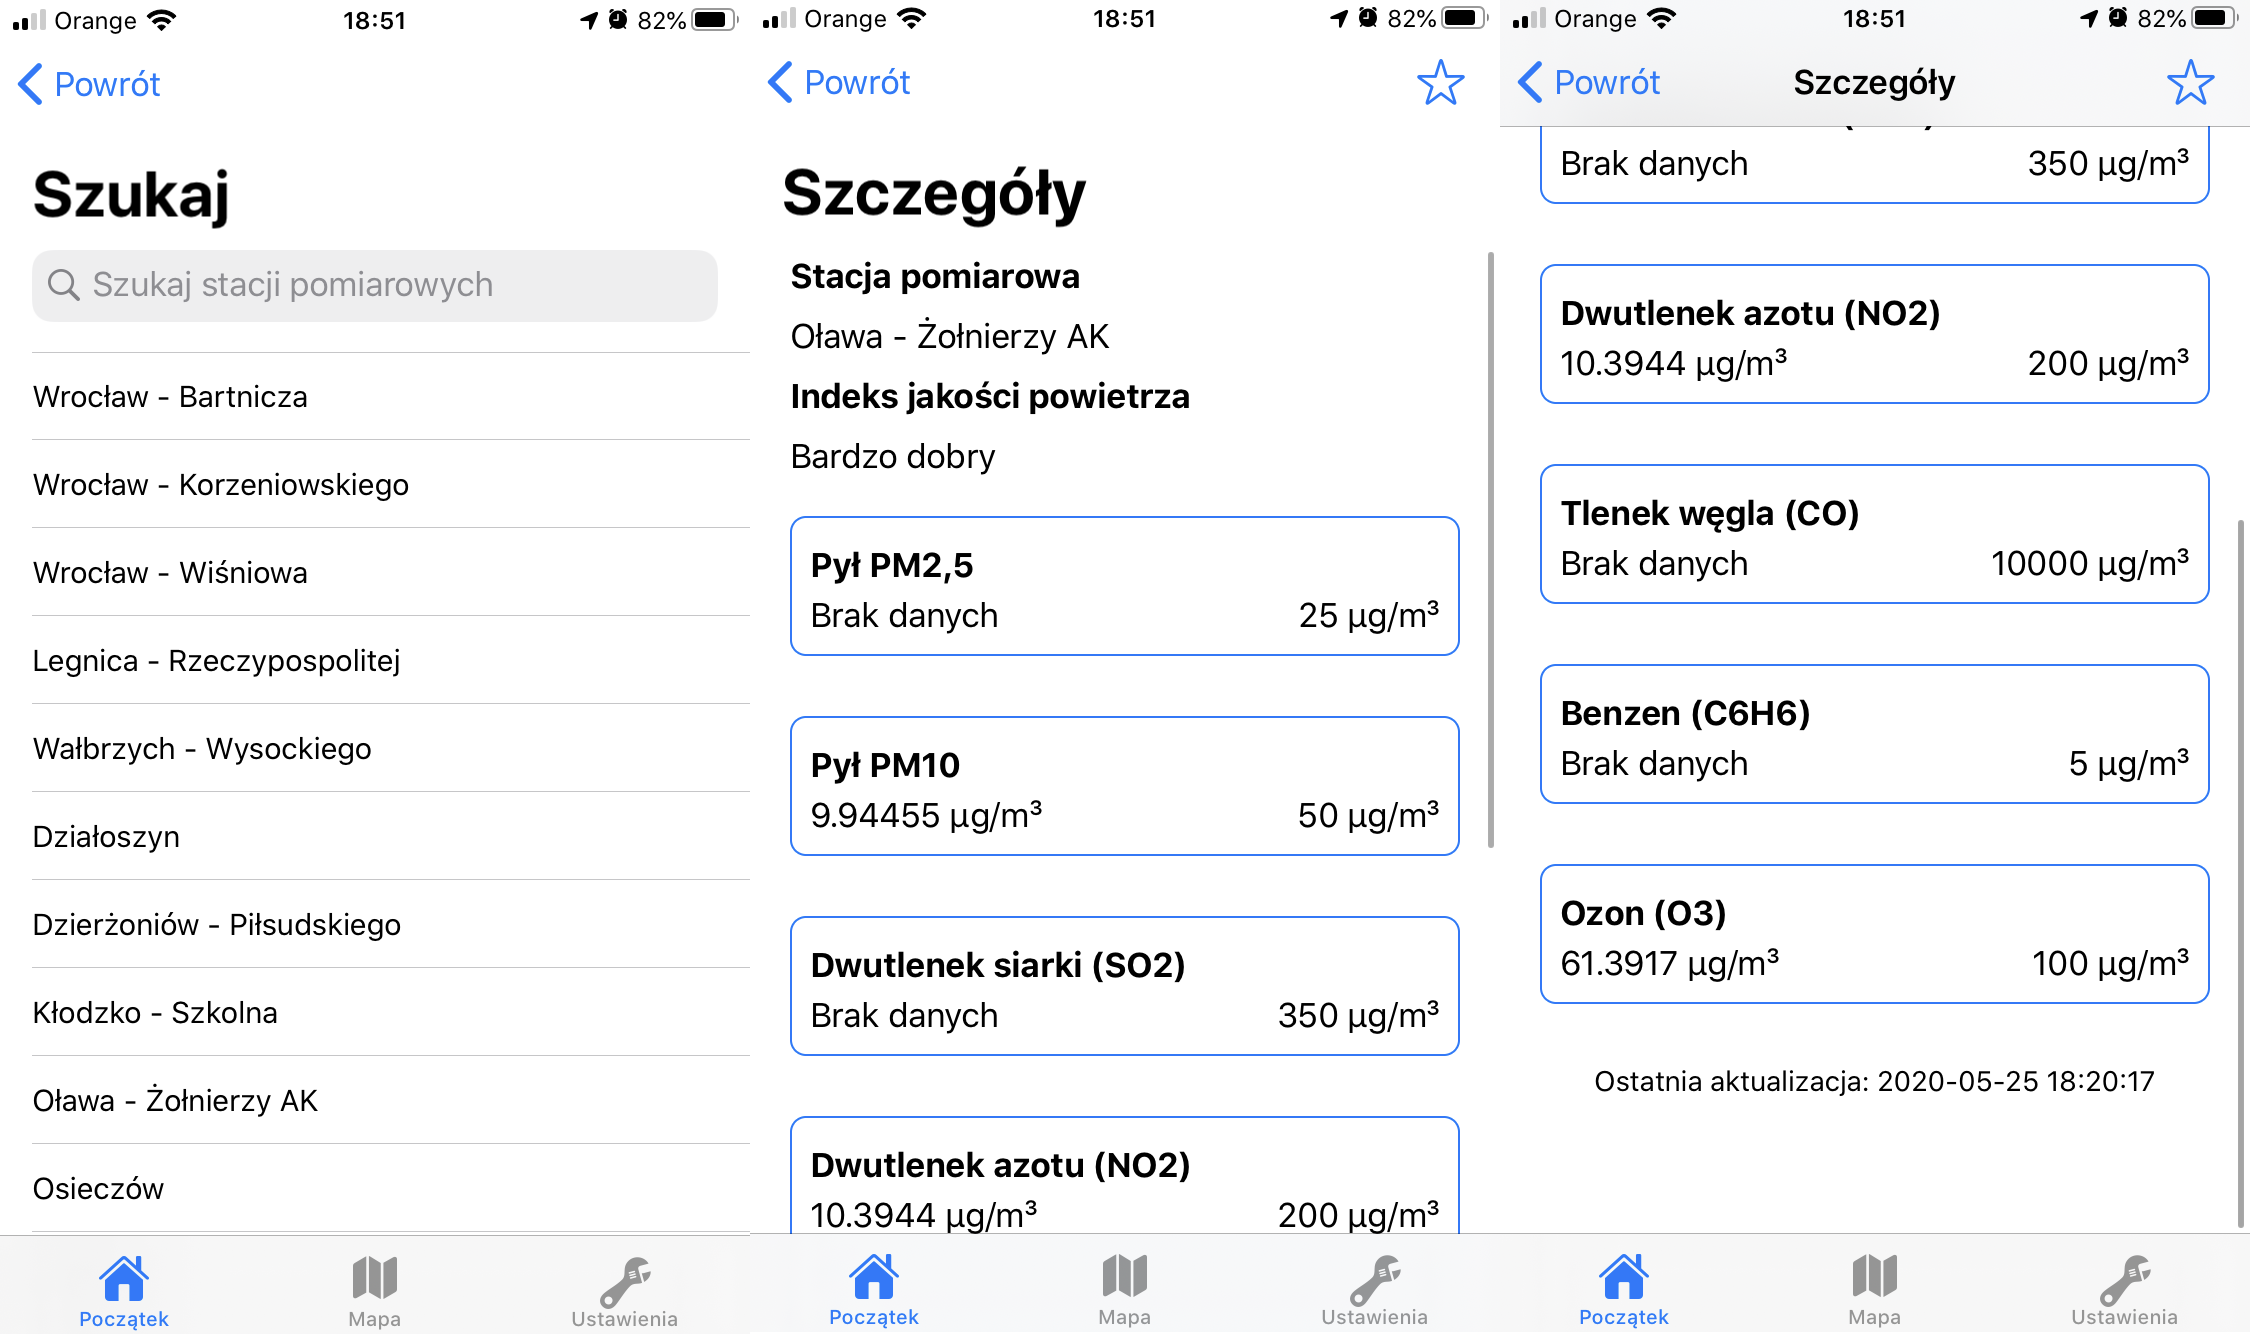
\includegraphics[width=1\columnwidth]{img/img2.PNG}
\caption{Wygląd wyszukiwarki stacji oraz szczegóły wybranej stacji pomiarowej} 
\end{figure}


Zakładka ustawienia na chwile obecną przechowuje informacje o autorze oraz o dostawy API, w przyszłości jednak planowane jest zaimplementowanie ustawień lokalizacji i powiadomień.

\section{Specyfikacja wewnętrzna}
\subsection{Struktura aplikacji}
Aplikacja zbudowana została z następujących kontrolerów i klas:
\begin{itemize}
 	\item Kontrolery widoków - odpowiedzialne za wyświetlanie danych zgodnie z ich przeznaczeniem, włączają się do tego klasy wyświetlające mapę, widok strony głównej, widok wyszukiwania stacji pomiarowych, widok ustawień, widok niestandardowych komórek w tabeli oraz widok szczegółów:
	\begin{itemize}
		\item \verb|MapViewController.swift|,
		\item \verb|HomeViewController.swift|, 
		\item \verb|SearchTableViewController.swift|,
		\item \verb|DetailsViewController.swift|,
		\item \verb|FavTableViewCell.swift|,
	\end{itemize}

	\item Klasy pomocnicze - występuje tylko jedna, odpowiedzialna za przechowywania adresów węzłów końcowych z API
	\begin{itemize}
		\item \verb|EndpointList.swift|,
	\end{itemize}

	\item Kontrolery logiki aplikacji - klasy, które realizują niezbędną logikę biznesową, czyli pobranie danych z odpowiedniego węzła końcowego API,  formatowanie danych z typu JSON na odpowiadające im struktury danych oraz przypisanie danych do odpowiednich struktur. W skład tej kategorii wchodzą klasy realizujące pobieranie danych:
	\begin{itemize}
		\item \verb|DataFetchProtocol.swift|,
		\item \verb|DataFetchController.swift|, 
		\item \verb|IdentifiedDataFetchController.swift|,
		\item \verb|DataPrepareController.swift|,
		\item \verb|DictionaryPrepareController.swift|,
	\end{itemize}

	\item Modele danych - odpowiednio przygotowane struktury danych, na których potem wykonywane są operacje. Modele zostały zaprojektowane na podstawie danych, jakie dostarcza API ``Jakość Powietrza'' GIOŚ. Zastosowane przeze mnie struktury danych:  
	\begin{itemize}
		\item \verb|StationModel.swift|,  
		\item \verb|SensorModel.swift|,
		\item \verb|IndexModel.swift|,
		\item \verb|ValueModel.swift|,
		\item \verb|CustomPinModel.swift|,
	\end{itemize}
\end{itemize}

Po uruchomieniu odpowiedniego widoku (np. kliknięcie w zakładkę mapy) kontroler widoku inicjalizuje kontroler logiki, który pobiera odpowiednie dane, które następnie ``opakowane'' zostają w odpowiednią strukturę danych. Ponieważ dane z API zwracane są w formacie JSON, kontroler ma za zadanie zdekodować je oraz ustawić ich odpowiedni format. Posiadając komplet danych, kontroler widoku jest w stanie wyświetlić na ekranie smartfona gotowy widok.
Dodatkowo, aplikacja posiada odpowiedni folder na zasoby (grafiki, ikony, itp.) o nazwie \verb|Assets.xcassets|, plik konfiguracyjny \verb|info.plist| (property list - który swoją składnią przypomina pliki XML) oraz specjalną tablicę do projektowania widoków oraz interakcji między nimi  \verb|Main.storyboard|.

Z powyżej listy interesującą pozycją może wydawać się plik konfiguracyjny, ponieważ do poprawnego działania aplikacji wymagane było dodanie następujących kluczy:
\begin{itemize}
 	\item ``Privacy - Location When In Use'' - komunikat podczas żądania lokalizacji od użytkownik
	\item ``App Tranport Security Settings'', ``Exception Domains'', ``NSIncludesSubdomains'', ``NSExceptionAllowInsecureHTTPLoads'' - biała lista adresów, z którymi aplikacja może się komunikować - bez tego klucza nie istaniała by możliwość by pobrać dane z publicznego API.
\end{itemize}

\subsection{Wzorce projektowe}
\subsubsection{MVC}
Szkielet aplikacji opiera się o bardzo popularny wzorzec MVC (Model - View - Controller) - a w przypadku tworzenia aplikacji w jezyku Swift nazywany też Cocoa MVC. Struktura aplikacji podzielona jest zatem na klasy związane z modelem danych (w którym znajdują się wszystkie pola odpowiedzialne za przechowywanie danych),  widok (elementy związane z wyświetlaniem danych), oraz kontrolery, które wykonują całą logikę aplikacji. Zaletą tego wzorca jest możliwość wielokrotnego użycia danych komponentów (np. tego samego modelu danych czy kontrolerów w wielu miejscach jednocześnie). W moim projekcie wielokrotnie używanymi elementami były klasy odpowiedzialne za pobranie danych z API oraz odpowiednie przetworzenie tych danych na modele.

\subsubsection{Delegacje}
W programowaniu aplikacji mobilnych w języku Swift bardzo popularnym wzorcem projektowym są delegacje (``Delegate pattern''). Delegacja jest wzorcem z programowania obiektowego, w którym obiekt zamiast sam wykonać pewną operację deleguje ją (zleca do wykonania) innemu obiektowi pomocniczemu (delegatowi). Następuje tu więc odwrócenie odpowiedzialności. Delegat jest odpowiedzialny za wykonanie zadania obiektu delegującego. Delegacje realizują podobne założenia do dziedziczenia jednak stosuje się je w miejscach, gdzie dziedziczenie może być niewygodne w implementacji.


\subsection{Biblioteki i API}
\subsubsection{Interfejs API portalu ``Jakość Powietrza'' GIOŚ}
Interfejs API portalu ``Jakość Powietrza''  GIOŚ umożliwia dostęp do danych dotyczących jakości powietrza w Polsce, wytwarzanych w ramach Państwowego Monitoringu Środowiska i gromadzonych w bazie JPOAT2,0

Dostęp do danych odbywa się poprzez zapytanie HTTP GET na podany w dokumentacji adres. Udostępniane dane zwracane są w formiacie JSON. Interfejs udostępnia dane o stacjach pomiarowych, stanowiskach pomiarowych (lista dostępnych stanowisk pomiarowych na wybranej stacji pomiarowej), dane pomiarowe oraz indeks jakości powietrza.

Lista adresów potrzebna do pobrania danych:
\begin{itemize}
 	\item \verb|http://api.gios.gov.pl/pjp-api/rest/station/findAll| - lista wszystkich stacji pomiarowych
	\item \verb|http://api.gios.gov.pl/pjp-api/rest/station/sensors/{stationId}| - lista dostępnych sensorów dla stacji pomiarowej na podstawie identyfikatora stacji
	\item \verb|http://api.gios.gov.pl/pjp-api/rest/data/getData/{sensorId}| - dane pomiarowe dla sensora o podanym w adresie id
	\item \verb|http://api.gios.gov.pl/pjp-api/rest/aqindex/getIndex/{stationId}| - indeks jakości powietrza na podstawie identyfikatora stacji pomiarowej
\end{itemize}
\subsubsection{Framework UIKit}
Framework pozwalający na tworzenie zaawansowanych widoków sterowanych zdarzeniami (``event-driven''). Powszechnie stosowany w aplikacjach na platformę iOS oraz tvOS. Wspiera animacje, multi-touch, dokumenty, drukowanie, zarządzanie elementami na ekranie (tekst, przyciski, itp), wyszukiwanie, dostępność oraz różne rozszerzenia.


\subsubsection{Framework MapKit}
Narzędzia pozwalające na wyświetlanie map wraz ze wszystkimi niezbędnymi elementami, takimi jak adnotacje, punkty, nakładki.

Implementacja wymaga sprawdzenia, czu urządzenie użytkownika posiada włączone usługi lokalizacyjne oraz czy użytkownik nadał uprawnienia do pobierania jego lokalizacji.

\subsubsection{Core Location}
Framework dostarczający takie usługi i funkcje jak aktualizacje lokacji użytkownika (z możliwością wybrania dokładności), obliczanie odległości pomiędzy dwoma punktami na mapie, monitoring danego obszaru, kompas itp. Framework zbiera dane przy użyciu Wi-Fi, GPS, Bluetooth, magnetometru oraz barometru.

\subsection{Kod źródłowy}
W podrozdziale ``Struktura aplikacji'' został szczegółowo omówiony podział aplikacji pod względem różnych zadań. W tym punkcie chciałbym doprecyzować znaczenie i działanie klas zawartych w projekcie.

\begin{itemize}
 	\item Kontrolery widoków
	\begin{itemize}
		\item \verb|HomeViewController.swift| - główna klasa widoku, która uruchamiana jest zaraz po włączeniu aplikacji. Dziedziczy ona klasy takie jak \verb|UIViewController|, \verb|UITableViewDataSource|,\newline \verb|UITableViewDelegate| oraz \verb|CLLocationManagerDelegate|. Przed załadowaniem widoku, klasa deleguje obiekty z klas, które dziedziczy, następnie sprawdza lokalizację użytkownika, pobiera listę wszystkich stacji i szuka tej w najbliższej okolicy. Obiekt klasy \verb|CLLocationManager| posiada funkcje, która na podstawie dwóch obiektów koordynatów wylicza odległość i przypisuje ją do obiektu(\verb|CLLocationDistance|). Zastosowano tutaj prosty algorytm wyszukiwania najmniejszej liczby. Po znalezieniu najbliższej stacji pomiarowej pobierany jest jej indeks i wyświetlany w odpowiednim miejscu. Kolejnym etapem jest pobranie tablicy z zakładkami. Zakładki przechowywane są w pamięci użytkownika w postaci tablicy indeksów (o typie \verb|Integer|). Mając listę stacji, aplikacja pobiera ich indeksy i zapisuje w tablicy. Tablica skorelowana jest z tabelą w widoku, w związku z czym wszystkie dane zamieniane są na komórki tabeli.
		\item \verb|MapViewController.swift| - klasa odpowiedzialna za widok mapy. Klasa rozszerzona jest (dziedziczy) o \verb|MKMapViewDelegate|, \newline \verb|CLLocationManagerDelegate| oraz \verb|UIViewController| w związku z którymi implementuje funkcje odpowiedzialne za aktualizację lokacji użytkownika (\verb|locationManager(...){...}|) oraz za przejście do szczegółów stacji pomiarowej po naciśnięciu w ikonę pineski (\verb|mapView(...){...}|). Przechowuje zmienne wraz ze wszystkimi stacjami pomiarowymi. Implementuje obiekt \newline \verb|CLLocationManager()|, który odpowiedzialny jest za pobranie lokalizacji użytkownika. Punktem wejsciowym klasy jest funkcja \verb|viewDidLoad(){...}|, która wykonuje zadania w następującej kolejności: pobiera wszystkie stacje pomiarowe (\verb|getStationArray()|), deleguje obiekt \verb|mapView| oraz \verb|locationManager|, sprawdza czy użytkownik wyraził zgodę na pobranie lokalizacji \newline(\verb|checkLocationServices()|) a na samym końcu wywołuje ona konstruktor klasy nadrzędnej (\verb|super.viewDidLoad()|)
		\item \verb|SearchTableViewController.swift| - klasa odpowiedzialna za wyświetlenie w tabeli listy wszystkich stacji pomiarowych, wyświetlenie oraz obsługa paska wyszukiwania oraz przejście do widoku szczegółów poprzez kliknięcie na daną komórkę w tabeli. Klasa rozszerzona jest przez: \verb|UITableViewController|, \newline \verb|UISearchControllerDelegate|, \verb|UISearchBarDelegate| oraz \newline \verb|UISearchResultsUpdating|. Konieczne było nadpisanie funkcji\newline  \verb|tableView(...){...}|, które wymagają podania ilości komórek w tabeli, uzupełnienie komórek danymi oraz przejście do szczegółów. Klasa odpowiedzialna za odświeżanie wyników wyszukiwania wymagała utworzenia funkcji \verb|updateSearchResult()|. Tak jak w każdym kontrolerze widoku, funkcją wejściową jest \verb|viewDidLoad(){}|, która tutaj pobiera dane ze stacji (\verb|getStationArray()|), inicjalizuje obiekt wyszukiwarki (\verb|searchBarSetup()|), wywołuje konsturktor klasy nadrzędnej (\verb|super.viewDidLoad()|) a na samym końcu odświeża dane tabeli (\verb|self.tableView.reloadData()|)
		\item \verb|DetailsViewController.swift| - dziedziczy tylko \verb|UIViewController|. Jej zadaniem jest pobranie danych na temat konkretnej stacji pomiarowej oraz wyświetlenie ich w odpowiednim miejscu. Przed załadowaniem widoku wywołuje funkcje \verb|getIndexLevel()|,\newline \verb|getSensors()|, \verb|getSensorValues()|
		\item \verb|FavTableViewCell.swift| - niestandardowy widok komórki w tabeli, dziedziczy on funkcjonalność po klasie bazowej \verb|UITableViewCell| jednak zawiera on dodatkowe pola jak \verb|NameLabel| oraz \verb|IndexLabel|, które są obiektami klasy \verb|UILabel|. Klasa nie implementuje sama w sobie żadnych dodatkowych funkcji.
	\end{itemize}

	\item Klasy pomocnicze (zawarte w folderze Helpers)
	\begin{itemize}
		\item \verb|EndpointList.swift| - Struktura danych zawierająca 4 zmienne statyczne typu String (allStations, index, sensors, sensorValue) wraz z adresami URL do odpowiedniego węzła końcowego. Nie wymaga inicjalizacji w innych klasach.
	\end{itemize}

	\item Kontrolery logiki aplikacji (zawarte w folderze LogicController)
	\begin{itemize}
		\item \verb|DataFetchProtocol.swift| - interfejs (w języku Swift interfejsy nazywane są protokołami) zawierające wzorzec dla klas pochodnych o tym jakie funkcje i zmienne powinny być przetwarzane. Mamy tutaj do czynienia ze zmienną \verb|endpoint| oraz funkcją \verb|fetchAllData|, która zwraca funkcję zwrotną (tzw. ``callback'').
		\item \verb|DataFetchController.swift| - implementacja powyższego protokołu, posiada konstruktor (funkcja \verb|init()|), który przypisuje wartość podaną jako argument do zmiennej \verb|endpoint|. Implementacja funkcji \verb|fetchAllData| skupia się na utworzeniu obiektu klasy \verb|URL| oraz wysłanie zapytania HTTP. Zwracana jest funkcja \verb|completion(data, res, err)|, której implementacja znajduje się już w poszczególnych kontrolerach i zazwyczaj opiera się na wywołaniu funkcji, która przygotowuje dane.
		\item \verb|IdentifiedDataFetchController.swift| - klasa dziedzicząca po \verb|DataFetchController|. Przyjmuje dodatkowy parametr \verb|idObject|, który dopisywany jest do adresu URL. Klasa ta różni się od klasy rodzica tym, że wysyła zapytania na adres, który wymaga podania parametru \verb|id|, np. do pobrania sensorów stacji o zadanym \verb|id|.
		\item \verb|DataPrepareController.swift| - klasa odpowiedzialna za zdekodowanie danych z formatu JSON na podany model danych. Model danych pobierany jest podczas inicjalizacji klasy (nie jako argument, klasa otrzymuje typ generyczny <T>), zatem jej tworzenie wygląda następująco: \newline \verb| let dataConverter = DataPrepareController<Station>()| \newline Klasa posiada wyłącznie jedną funkcję \verb|prepareData(data: Data)|, która zwraca tablicę obiektów, podanych na początku.
		\item \verb|DictionaryPrepareController.swift| - klasa blizniacza do DataPrepareController, tylko zamiast tablicy obiektów, dekoduje ona pojedyńczy obiekt. Związane jest to z faktem, że dane w formacie JSON mogą zostać zwrócone jako tablica (wówczas dane zawarte są w kwadratowych nawiasach \verb|[ ... ]|) bądź jako poszczególny obiekt (w języku Swift nazywany ``Dictionary'') - wtedy dane JSON umieszczone są w klamrach \verb|{ ... }|.
	\end{itemize}

	\item Modele danych
	\begin{itemize}
		\item \verb|StationModel.swift| - model zawierający struktury danych stacji (id, nazwa stacji, współrzędne geograficzne) oraz struktury miasta (id, nazwa) oraz strukture z danymi gminy (nazwa gminy, nazwa powiatu, nazwa województwa)
		\item \verb|SensorModel.swift| - model przechowujący id i id stacji pomiarowej.
		\item \verb|IndexModel.swift| - struktura danych zawierająca informacje o id, dacie pomiaru oraz nazwie indeksu.
		\item \verb|ValueModel.swift| - struktura zawierająca w sobie tablicę obiektów z wartościami (data, wartość) dla danego stanowiska pomiarowego reprezentowanego zmienną \verb|key|
		\item \verb|CustomPinModel.swift| - klasa dziedzicząca po klasie\newline \verb|MKPointAnnotation|. Dodaje do swojej struktury zmienną z obiektem typu \verb|Station|
	\end{itemize}
\end{itemize}


\subsection{Uruchomienie aplikacji w środowisku deweloperskim}
Do uruchomienia aplikacji wymagany jest komputer firmy Apple z zainstalowaną aplikacją Xcode. Po ściągnięciu i otwarciu projektu wystarczy wybrać urządzenie z listy na górnym pasku a następnie wcisnąc przycisk odpowiedzialny za uruchomienie. Jeżeli wybrane urządzenie nie jest fizycznym smartfonem, uruchomiony zostanie emulator, który w ciągu kilku minut zainicjalizuje naszą aplikację. Warto zwrócić uwagę, że korzystając z emulatora można doświadczać problemów z poprawnym wyświetlaniem lokalizacji użytkownika, dlatego w celu przetestowania aplikacji sugerowane jest użycie fizycznego urządzenia.


\section{Podsumowanie}
\subsection{Uwagi}
Podczas tworzenia aplikacji napotkałem wiele trudności i problemów, które wymagały zasięgnięcia porady w internecie. Niektóre z tych problemów wynikają ze specyfiki języka Swift (który bazuje na Objective-C) lub z nawyków, które nabyłem programując w innych technologiach.

Język Swift posiada bardzo specyficzną składnię czerpiącą wiele z nowoczesnych języków. Ciężko było przywyknąć mi do nietypowych deklaracji zmiennych, np. \verb|let| oraz \verb|var|, które w jęzuku JavaScript nie różnią się za bardzo od siebie - tutaj jednak, ta pierwsza definiuje nam stałą wartość, której nie można już później zmienić, druga definicja to deklaracja zwykłej zmiennej. Ciekawą rzeczą, którą poznałem jest również wyrażenie \newline \verb|guard [wyrażenie] else { kod aplikacji }|. Jest to nic innego jak \verb|if|, który wykona kod w klamrach tylko wtedy, gdy wartość wyrażenia przyjmie fałsz. Będąc przy temacie składni nie może zabraknąć informacji o tzw. ``optional chaining'', które w kwietniu 2020 dopiero zostało wprowadzone w języku JavaScript. Polega to na tym, że nie musimy każdorazowo sprawdzać instrukcją \verb|if| czy nasza zmienna, do której chcemy się odnieść istnieje Wykorzystuje się do tego znak zapytania. Pozwala to zredukować ilość nadmiarowego kodu. Przykład:\newline
Wyrażenie \verb|let sensors = obj.station && obj.station.sensors| \newline
Możemy zastąpić poprzez: \verb|let sensors = obj.station?.sensors|\newline Jest to ułatwienie, które w ostatnim czasie jest implementowane również w innych językach.


Obsługa asynchronicznych funkcji też znacznie różni się od tych, do których przyzwyczaił mnie JavaScript. Pobierając dane z API oczekuje się, że widok wygeneruje się dopiero po tym jak wygenerowana zostanie odpowiedź. We wspomnianym wcześniej JavaScripcie możliwe jest to za pomocą wyrażeń \verb|async| oraz \verb|await|. Tutaj niestety sytuacja jest dużo trudniejsza. W języku Swift wymagane jest zaimplementowanie funkcji \verb|completion|. Oficjalna dokumentacja określa to jako ``funkcje domknięcia (closures)'' i przyrównuje je do bloków w Objective-C lub wyrażeń lambda w języku Java.


API GIOŚ, które jest stosowane w aplikacji zwraca typy danych, które nie są obsługiwane w języku Swift, np \verb|null|. Wymaga to dodatkowej obsługi niektórych żądań i wymusza na programiście zaimplementowanie dodatkowych funkcji do konwersji null na obsługiwany przez kompilator \verb|nil|. Kolejnym przykładem mogą być dane dotyczące współrzędnych geograficznych, można by spodziewać się, że skoro identyfikatory przesyłane są jako Integer, to współrzędne będą typu miały typ Double lub inny zmiennoprzecinkowy typ. Niestety, większość danych (łącznie z liczbowymi) przesyłane są jako zwykły String. Implikuje to dodatkową konwersję w kodzie. Dodatkowo, narzędzia udostępniane przez Główny Inspektorat Ochrony Środowiska nie do końca spełniają wymogi aplikacji REST. Brakuje pewnej konsekwencji w nazwach węzłów końcowych, które powinny być rzeczownikami w liczbie pojedyńczej, np. adres \verb|...rest/station/findAll| powinien zostać zastąpiony przez \verb|...rest/station|. Utrudnieniem podczas korzystania z interfejsu był również fakt, że API nie zwraca pełnego kompletu danych potrzebnych do obsługi funkcjonalności w aplikacji. Nie istnieje węzeł końcowy, który zwracałby dane stacji, sensorów, wartości pomiarowych i indeksu powietrza jednocześnie. Zostało to rozbite na cztery różne adresy: najpierw musimy znaleźć interesującą nas stację, następnie na podstawie id stacji pobieramy listę dostępnych dla niej sensorów, posiadająć id dla sensorów wysyłamy żądanie HTTP by pobrać ich wartości a na samym koncu odpytujemy system na podstawie id stacji o indeks jakości powietrza. Według mnie system ten mógłby być bardziej przemyślany.


W początkowych założeniach projektowych można było wyszczególnić punkt odnoszący sie do powiadomień push, w związku z którymi użytkownik miał otrzymywać informacje za każdym razem, gdy jakość powietrza na stacji pomiarowej uległa pogorszeniu. Niestety, implementacja ten fukcji była niemożliwa z dwóch powodów:
\begin{enumerate}
	\item Wymagany byłby osobny serwer, który musiałby porównywać jakość powietrza z poprzednich godzin z aktualną i jeżeli ta uległa by pogorszeniu, wysłać powiadomienie do użytkownika. Jest to najmniejszy problem, ponieważ taki serwer można utworzyć w kilka godzin.
	\item Do wysyłania powiadomień push należy mieć konto deweloperskie, które kosztuje około 400 złotych. Fakt ten całkowicie uniemożliwił mi realizację tego założenia.
\end{enumerate}


Ostatnią trudnością w programowaniu aplikacji na iOS jest fakt, że można je tworzyć tylko na urządzeniach Apple. Według mnie praca na laptopie i małym ekranie jest dużo bardziej męcząca niż wykonywanie tego samego zadania na komputerze stacjonarnym.

\subsection{Błędy}
Jak w każdym projekcie, naturalną rzeczą są błędy. W mojej aplikacji mogę wyróżnić błędy wynikające ze źle dobranej przeze mnie architektury. Jednym z błędów jest brak wyświetlania się listy wszystkich dostępnych stacji w widoku wyszukiwania (występuje w ok. 1/10 przypadków). Błąd wynika z tego, że widok jest generowany zanim dane zostaną pobrane poprzez protokół HTTP i załadowane do tablicy. Pomimo próby wyeliminowania błędu (poprzez kilkukrotne odświeżanie widoku) nie udało mi się do końca wyeliminować problemu. Błąd nie występowałby, gdybym w założeniach projektowych wybrał architekturę MVVM (Model-View-ViewModel), gdyż ta implementuje klasy i funkcje, które odświeżają widok za każdym razem, gdy dane oznaczone poprzez adnotację \verb|@Observable| zostaną zmienione.

\subsection{Możliwość dalszego rozwoju}
Aplikacja na chwile obecną obsługuje tylko Polskę, jednakże dzięki zastosowaniu interfejsów (w jęzuku Swift nazywanych protokołami) można zaimplementować funkcję do pobierania danych również z innych rejonów świata. Wymaga to jedynie dostosowania wyników zapytań do modelów danych, którymi posługuje się aplikacja. Funkcje pobierania danych z API przyjmują argumenty typu generycznego, w związku z czym można do nich przesłać modele danych innych, niż zostały obecnie zaimplementowane.

\subsection{Wnioski}
Projektowanie aplikacji na iOS mogę porównać do budowania domu. Pierwszy dom buduje się dla wroga, drugi dla przyjaciela a trzeci dla siebie. Gdybym musiał napisać kolejną aplikację w tej technologii, zdecydowanie wybrałbym inny wzorzec projektowy, np. MVVM (Model-View-ViewModel) zamiast próbować implementować Cocoa MVC (żartobliwie nazywany Massive View Controller).  Niestety, założenia, które przyjąłem na samym początku projektu okazały się być niewystarczające w kontekście programowania dobrych aplikacji, jednakże ich zmiana wiązała by się z potrzebą poświęcenia dużej ilości czasu, którego niestety mi brakło.


Zdecodywanie pozytywnym zaskoczeniem podczas tworzenia projektu okazał się być debugger, którego nie trzeba było w żaden sposób konfigurować, był on zintegrowany z narzędziem XCode, z którego korzystałem. W żadnym innym projekcie tak często nie korzystałem z tego narzędzia.


Podczas pracy nad aplikacją poznałem znaczenie niektórych wzorców projektowych, dodatkowo zauważyłem, że programowanie aplikacji webowych różni się w znaczącym stopniu od programowania aplikacji mobilnych. Sama technologia jednak wydaje się być niesprzyjająca dla nowych użytkowników, dlatego według mnie, żeby zacząć przygodę z językiem Swift trzeba mieć solidne podstawy w programowaniu innych (najlepiej nowoczesnych) języków programowania. Swift skupia się na niektórych wzorcach w sposób bardziej znaczący, niż inne technologie, z którymi miałem do czynienia.

Przedsięwzięcie to okazało się być bardziej czasochłonne niż się spodziewałem, wymagało zapoznania się z dokumentacją wielu frameworków oraz ciągłym szukaniem rozwiązań problemów, z którymi dotychczas się nie spotkałem.


\newpage
\addcontentsline{toc}{section}{Spis rysunków}
\listoffigures
\newpage

\begin{thebibliography}{9}
\addcontentsline{toc}{section}{Literatura}
\bibitem{uikit}
\verb|https://developer.apple.com/documentation/uikit|
\bibitem{mapkit}
\verb|https://developer.apple.com/documentation/mapkit/|
\bibitem{cllocationmanager}
\verb|https://developer.apple.com/documentation/corelocation/cllocationmanager|
\bibitem{delegationpatter}
\verb|http://programowanie.siminskionline.pl/resource/wp/ood_strategy.pdf|
\bibitem{ltba}
\verb|https://www.letsbuildthatapp.com/|



\end{thebibliography}
\end{document}